\documentclass[10pt]{beamer}
\usetheme{Goettingen}

\usepackage[utf8]{inputenc}
\usepackage[T1]{fontenc}
% clashes with neural net figure
%\usepackage[french]{babel}

\usepackage{pgfplots}

\usepackage{algorithmicx}
\usepackage{algpseudocode}

%\usepackage{frpseudocode}

\usepackage{caption}

\newcommand{\kw}[1]{\textrm{#1}}

\usepackage{forest}

%\usepackage{scrextend}
%\changefontsizes{7.5pt}

\usefonttheme[onlymath]{serif}

\usepackage{xcolor}
\usepackage{graphicx}
\usepackage{amsmath}
\usepackage{amssymb} % pour les ensembles NN
\usepackage{mathrsfs} % pour les hypothèses de récurrences \PP
\setlength{\unitlength}{1mm}
%\usepackage{enumitem}
\usepackage{cancel}

\usepackage{neuralnetwork}

%\usepackage{fancyhdr}
\usepackage{multicol}

\usepackage{multicol}
\usepackage{minted}
\setminted{
    %linenos=true,
    breaklines=true,
    %breakanywhere=true,
    encoding=utf8,
    fontseries=heiti,
    % autogobble=true,
    %frame=lines
}

\usepackage{booktabs}
\usepackage{tabularx}
\usepackage{array,collcell}
\newcommand\AddLabel[1]{%
  \refstepcounter{equation}% increment equation counter
  (\theequation)% print equation number
  \label{#1}% give the equation a \label
}
\newcolumntype{M}{>{\hfil}X<{\hfil}} % mathematics column
%\newcolumntype{M}{>{\hfil$\displaystyle}X<{$\hfil}} % mathematics column
%\newcolumntype{L}{>{\collectcell\AddLabel}r<{\endcollectcell}}
\renewcommand\tabularxcolumn[1]{m{#1}}% for vertical centering text in X column

\usepackage{graphicx} % for \resizebox

\usepackage{tikz}
\usetikzlibrary{matrix,chains,positioning,decorations.pathreplacing,arrows,shapes, calc,shadows,arrows.meta}

\usepackage{tkz-graph}
\tikzset{EdgeStyle/.append style = {->}}
\tikzset{LabelStyle/.style= {draw,
fill = white,
text = black}}

\newcommand*\keystroke[1]{%
  \tikz[baseline=(key.base)]
    \node[%
      draw,
      fill=white,
      drop shadow={shadow xshift=0.25ex,shadow yshift=-0.25ex,fill=black,opacity=0.75},
      rectangle,
      rounded corners=2pt,
      inner sep=1pt,
      line width=0.5pt,
      font=\scriptsize\sffamily
    ](key) {#1\strut}
  ;
}

\newcommand*\circled[1]{\tikz[baseline=(char.base)]{
            \node[shape=circle,draw,inner sep=1pt] (char) {#1};}}

\usepackage{etoolbox} % for \ifnumcomp
\usepackage{listofitems} % for \readlist to create arrays

\tikzset{>=latex} % for LaTeX arrow head
\colorlet{myred}{red!80!black}
\colorlet{myblue}{blue!80!black}
\colorlet{mygreen}{green!60!black}
\colorlet{mydarkred}{myred!40!black}
\colorlet{mydarkblue}{myblue!40!black}
\colorlet{mydarkgreen}{mygreen!40!black}
\tikzstyle{node}=[very thick,circle,draw=myblue,minimum size=22,inner sep=0.5,outer sep=0.6]
\tikzstyle{connect}=[->,thick,mydarkblue,shorten >=1]
\tikzset{ % node styles, numbered for easy mapping with \nstyle
  node 1/.style={node,mydarkgreen,draw=mygreen,fill=mygreen!25},
  node 2/.style={node,mydarkblue,draw=myblue,fill=myblue!20},
  node 3/.style={node,mydarkred,draw=myred,fill=myred!20},
}
\def\nstyle{int(\lay<\Nnodlen?min(2,\lay):3)} % map layer number onto 1, 2, or 3

% ensembles N,Z,Q,D,R,C
\DeclareMathOperator{\NN}{\mathbb{N}}
\DeclareMathOperator{\ZZ}{\mathbb{Z}}
\DeclareMathOperator{\QQ}{\mathbb{Q}}
\DeclareMathOperator{\DD}{\mathbb{D}}
\DeclareMathOperator{\RR}{\mathbb{R}}
\DeclareMathOperator{\CC}{\mathbb{C}}
\DeclareMathOperator*{\argmax}{\arg\!\max}

\newcommand*\colvec[3][]{
    \begin{pmatrix}\ifx\relax#1\relax\else#1\\\fi#2\\#3\end{pmatrix}
}

\newcommand*\linvec[3][]{
    \left(\ifx\relax#1\relax\else#1,\fi#2, #3\right)
}

\title{TIPE 2024}
\subtitle{Apprendre à une intelligence artificielle à jouer à Snake en utilisant un algorithme génétique}
\author{Marilou Bernard de Courville}
\institute{Lycée Charlemagne}
\date{\today}

\setbeamertemplate{footline}[frame number]

\begin{document}

\begin{frame}
    \titlepage
\end{frame}

%\begin{frame}
%    \frametitle{Table des matières}
%    \tableofcontents
%\end{frame}

\section{Principe}

\subsection{Introduction}

\begin{frame}
\frametitle{Introduction}
\framesubtitle{Problématique et pertinence au regard du thème de l'année}
\begin{itemize}
\item \textbf{Le jeu de Snake:} piloter un serpent sur une grille dans le but de
manger des pommes, sans rentrer dans les murs ni se replier sur
soi-même.
\item \textbf{Objectif:} mettre en place une intelligence
artificielle pouvant jouer efficacement au jeu de Snake, apprenant de manière autonome.
\item \textbf{Le moyen d'y parvenir:} utiliser un algorithme génétique,
qui s'inspire de l'évolution naturelle pour entraîner un réseau de neurone opérant les décisions de mouvement
du serpent dont les entrées sont des paramètres de vision.
\end{itemize}
\end{frame}

\subsection{Le jeu de Snake}

\begin{frame}
\frametitle{Le jeu de Snake}
\framesubtitle{Brève histoire et règles du jeu}
\begin{columns}[T]
\begin{column}{0.70\textwidth}
\footnotesize
\textbf{Origine:} borne d'arcade \textit{Blockade}, créée par Gremlin en 1976, popularisé par Nokia en 1997 sur mobile

\vspace{0.2cm}
\textbf{Règles du jeu:}
\begin{itemize}
\footnotesize
\item Le serpent débute avec une longueur initiale donnée sur un échiquier entouré d'un mur et contenant une pomme.
\item L'objectif est de le faire grandir en mangeant des pommes.
\item Chaque pomme consommée augmente sa longueur d'une unité et fait apparaître une nouvelle pomme à un emplacement aléatoire.
\item Le joueur dirige le serpent à l'aide des touches directionnelles du clavier \keystroke{$\leftarrow$}\keystroke{$\uparrow$}\keystroke{$\downarrow$}\keystroke{$\rightarrow$}.
\item Le jeu se termine si le serpent heurte un mur ou son propre corps.
\item Le score du joueur est égal au nombre de pommes mangées.
\end{itemize}
\end{column}
\begin{column}{0.26\textwidth}
\begin{figure}
\centering
\vspace{-1.7cm}
%\hspace{-0.6cm}
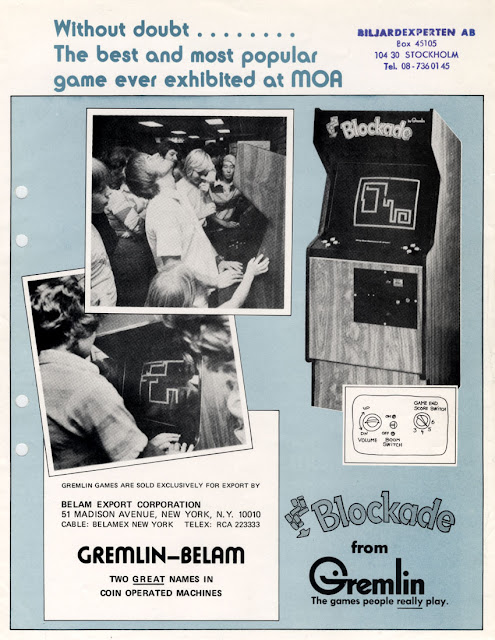
\includegraphics[width=1\textwidth]{blockade.jpg}
\end{figure}

\begin{figure}
\vspace{-0.4cm}
%\hspace{-0.6cm}
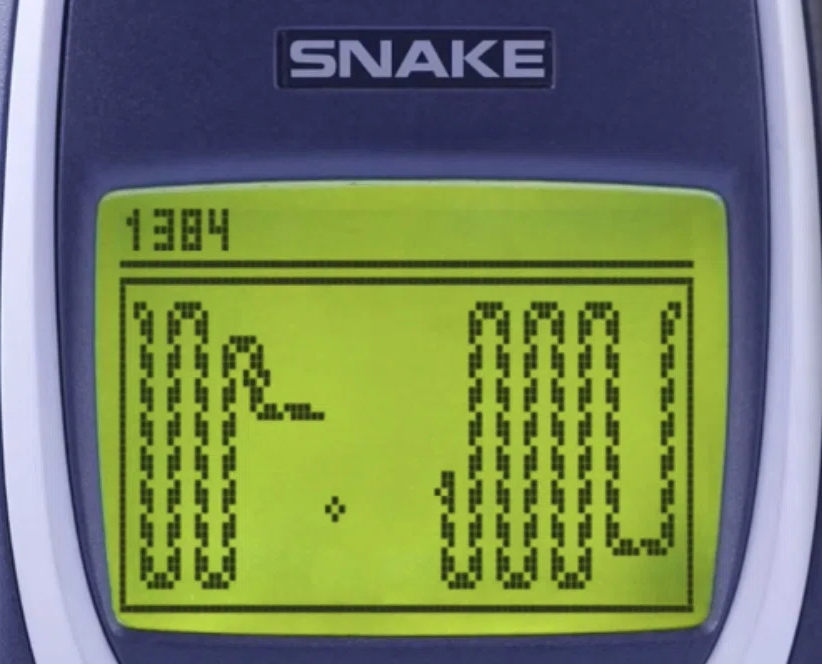
\includegraphics[width=0.97\textwidth]{snake_nokia.png}
\end{figure}

\begin{figure}
\vspace{-0.4cm}
%\hspace{-0.6cm}
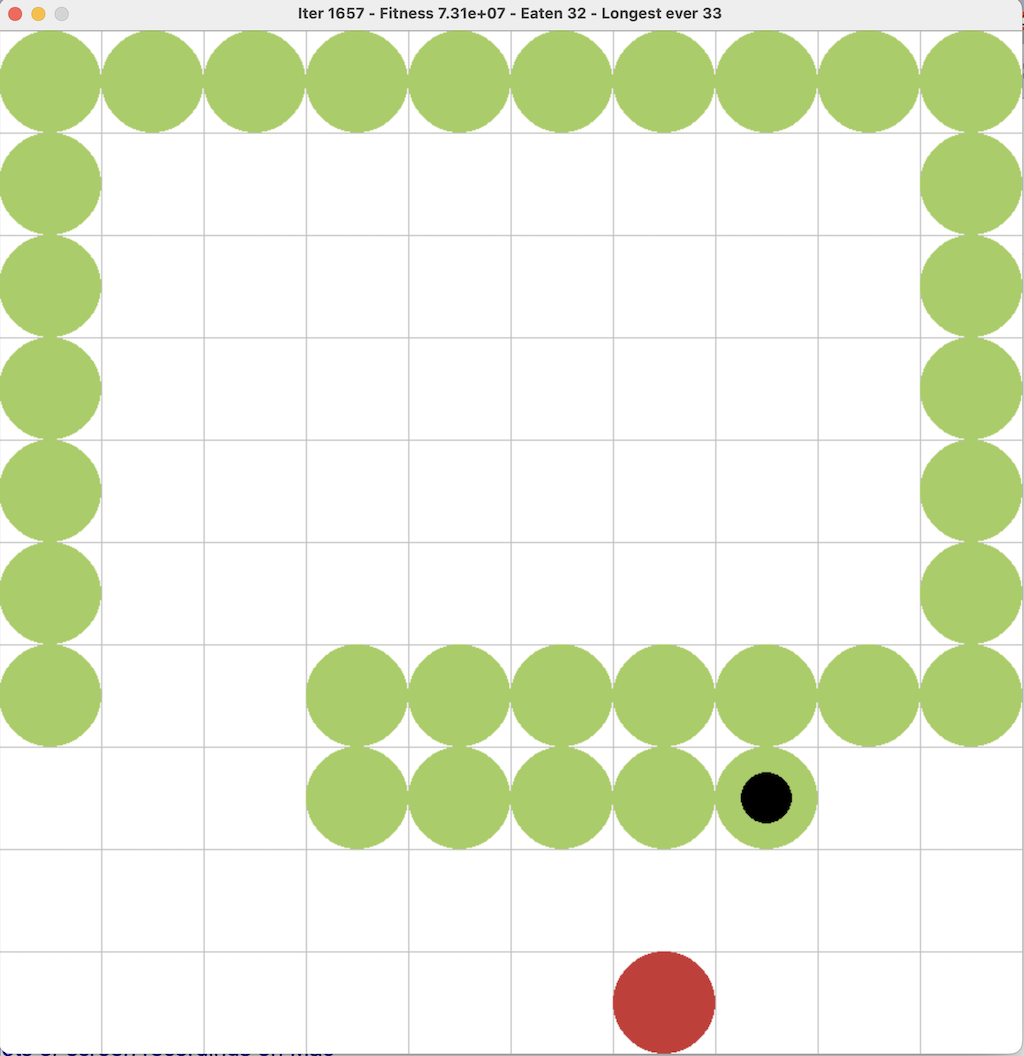
\includegraphics[width=1\textwidth]{snake_game.png}
\end{figure}
\end{column}
\end{columns}
\end{frame}

\section{Réseau de neurones}

\subsection{Déplacement}

\begin{frame}
  \frametitle{Déplacer le serpent}
  \framesubtitle{Grâce à un réseau de neurones}

  \begin{columns}[T]
  \begin{column}{0.60\textwidth}
  \footnotesize

  \textbf{Idée:} utiliser un réseau de neurones multicouches à propagation avant pour déterminer le mouvement du serpent.
  \begin{itemize}
    \item Entrées: paramètres de vision.
    \item Sorties: les directions \keystroke{$\leftarrow$}\keystroke{$\uparrow$}\keystroke{$\downarrow$}\keystroke{$\rightarrow$}.
  \end{itemize}

  \vspace{0.2cm}
  \textbf{Modélisation d'un neurone:} somme pondérée des entrées par un poids synaptique auquel on ajoute un biais. Sortie générée par une fonction d'activation non linéaire.
  \begin{align*}
    %\mathbf{x} & = \colvec[x_1]{\vdots}{x_n}, \mathbf{h} = \colvec[h_1]{\vdots}{h_n} \\
    \mathbf{x} & = \linvec[x_1]{\cdots}{x_n}^\intercal, \mathbf{h} = \linvec[h_1]{\cdots}{h_n}^\intercal \\
               y & = \sigma\left(\mathbf{h}^\intercal \mathbf{x} + b\right)  \\
  \end{align*}

  \vspace{-0.4cm}
  \textbf{Généralisation à un réseau multicouches:} modélisation matricielle avec fonction vectorielle $\sigma$
  \begin{equation*}
  \resizebox{\textwidth}{!}{
  $\begin{pmatrix}
    y_{1} \\[0.3em]
    y_{2} \\
    \vdots \\
    y_{m}
  \end{pmatrix}
    =
    \sigma\left[
    \begin{pmatrix}
    h^{(2)}_{1,1} & h^{(2)}_{1,2} & \ldots & h^{(2)}_{1,k} \\
    h^{(2)}_{2,1} & h^{(2)}_{2,2} & \ldots & h^{(2)}_{2,k} \\
    \vdots & \vdots & \ddots & \vdots \\
    h^{(2)}_{m,1} & h^{(2)}_{m,2} & \ldots & h^{(2)}_{m,k}
    \end{pmatrix}
    \sigma\left(
  \begin{pmatrix}
    h^{(1)}_{1,1} & h^{(1)}_{1,2} & \ldots & h^{(1)}_{1,n} \\
    h^{(1)}_{2,1} & h^{(1)}_{2,2} & \ldots & h^{(1)}_{2,n} \\
    \vdots & \vdots & \ddots & \vdots \\
    h^{(1)}_{k,1} & h^{(1)}_{k,2} & \ldots & h^{(1)}_{k,n}
    \end{pmatrix}
    \begin{pmatrix}
    x_{1} \\[0.3em]
    x_{2} \\
    \vdots \\
    x_{n}
    \end{pmatrix}
    +
    \begin{pmatrix}
    b_{1}^{(1)} \\[0.3em]
    b_{2}^{(1)} \\
    \vdots \\
    b_{k}^{(1)}
    \end{pmatrix}
    \right)
    +
    \begin{pmatrix}
    b_{1}^{(2)} \\[0.3em]
    b_{2}^{(2)} \\
    \vdots \\
    b_{m}^{(2)}
    \end{pmatrix}
    \right] 
  $}
  \end{equation*}
  \textbf{Décision de direction:} celle qui a la plus grande valeur de sortie.

  \end{column}
  \begin{column}{0.4\textwidth}
  \begin{figure}
  \vspace{-1cm}\hspace{-0.6cm}
  \centering
  \resizebox{\textwidth}{!}{
  % neural network pipeline
  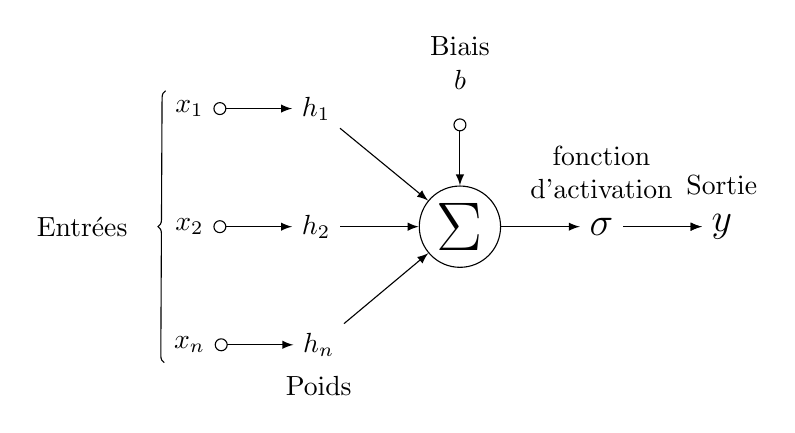
\begin{tikzpicture}[
      % define styles
      init/.style={
           draw,
           circle,
           inner sep=2pt,
           font=\Huge,
           join = by -latex
      },
      squa/.style={
          font=\Large,
          join = by -latex
      }
  ]
  % Top chain x1 to w1
  \begin{scope}[start chain=1]
      \node[on chain=1] at (0,1.5cm)  (x1) {$x_1$};
      \node[on chain=1,join=by o-latex] (w1) {$h_1$};
  \end{scope}
  % Middle chain x2 to output
  \begin{scope}[start chain=2]
      \node[on chain=2] (x2) {$x_2$};
      \node[on chain=2,join=by o-latex] {$h_2$};
      \node[on chain=2,init] (sigma) {$\displaystyle\Sigma$};
      \node[on chain=2,squa,label=above:{\parbox{2cm}{\centering fonction \\ d'activation}}]   {$\sigma$};
      \node[on chain=2,squa,label=above:Sortie,join=by -latex] {$y$};
  \end{scope}
  % Bottom chain x3 to w3
  \begin{scope}[start chain=3]
      \node[on chain=3] at (0,-1.5cm)
      (x3) {$x_n$};
      \node[on chain=3,label=below:Poids,join=by o-latex]
      (w3) {$h_n$};
  \end{scope}
  % Bias
  \node[label=above:\parbox{2cm}{\centering Biais \\ $b$}] at (sigma|-w1) (b) {};
  % Arrows joining w1, w3 and b to sigma
  \draw[-latex] (w1) -- (sigma);
  \draw[-latex] (w3) -- (sigma);
  \draw[o-latex] (b) -- (sigma);
  % left hand side brace
  \draw[decorate,decoration={brace,mirror}] (x1.north west) -- node[left=10pt] {Entrées} (x3.south west);
  \end{tikzpicture}
  }
  \vspace{-0.2cm}
  \caption*{\tiny Fonctionnement d'un neurone}
  \end{figure}

  \begin{figure}
  \vspace{-0.8cm}\hspace{-0.6cm}
  \centering
  \resizebox{\textwidth}{!}{
  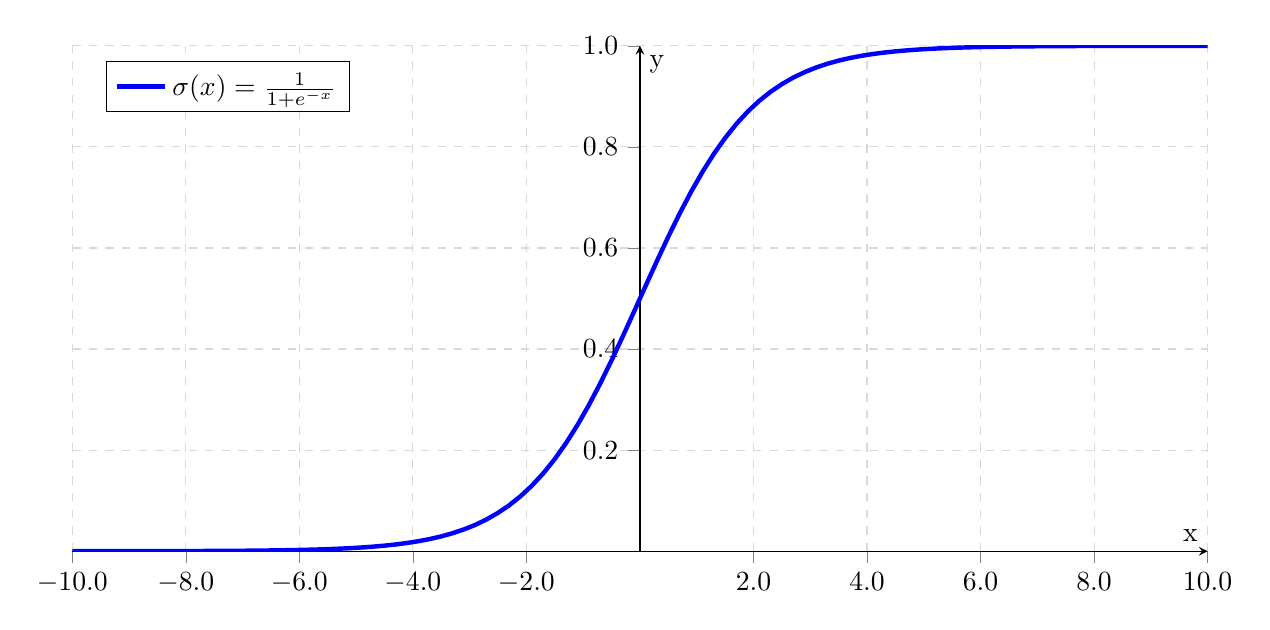
\begin{tikzpicture}
      \begin{axis}[
        legend pos=north west,
          axis x line=middle,
          axis y line=middle,
          x tick label style={/pgf/number format/fixed,
                              /pgf/number format/fixed zerofill,
                              /pgf/number format/precision=1},
          y tick label style={/pgf/number format/fixed,
                              /pgf/number format/fixed zerofill,
                              /pgf/number format/precision=1},
          grid = major,
          width=16cm,
          height=8cm,
          grid style={dashed, gray!30},
          xmin=-10,     % start the diagram at this x-coordinate
          xmax= 10,    % end   the diagram at this x-coordinate
          ymin= 0,     % start the diagram at this y-coordinate
          ymax= 1,   % end   the diagram at this y-coordinate
          %axis background/.style={fill=white},
          xlabel=x,
          ylabel=y,
          tick align=outside,
          enlargelimits=false]
        % plot the function
        \addplot[domain=-50:50, blue, ultra thick, samples=500] {1/(1+exp(-x))};
        \addlegendentry{$\sigma(x)=\frac{1}{1+e^{-x}}$}
      \end{axis}
  \end{tikzpicture}
  } % End of \resizebox
  \vspace{-0.2cm}
  \caption*{\tiny Fonction d'activation sigmoide}
  \end{figure}

  \begin{figure}
  \vspace{-0.8cm}\hspace{-0.6cm}
  \centering
  \resizebox{\textwidth}{!}{
  % NEURAL NETWORK
  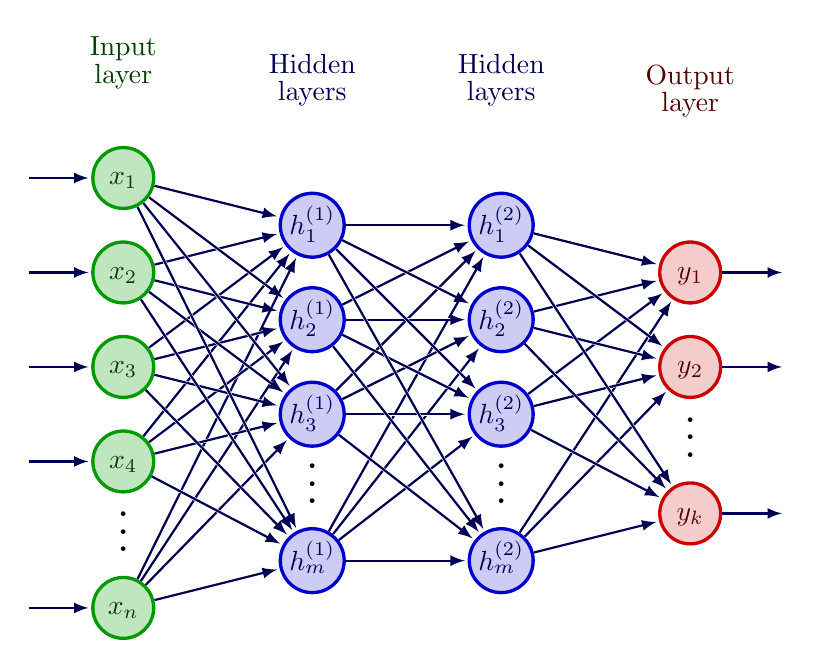
\begin{tikzpicture}[x=2.4cm,y=1.2cm]
  %  \readlist\Nnod{4,3,2} % array of number of nodes per layer
    \readlist\Nnod{5,4,4,3}
    \readlist\Nstr{n,m,k} % array of string number of nodes per layer
    \readlist\Cstr{x,h^{(\prev)},y} % array of coefficient symbol per layer
    \def\yshift{0.55} % shift last node for dots

    % LOOP over LAYERS
    \foreachitem \N \in \Nnod{
      \def\lay{\Ncnt} % alias of index of current layer
      \pgfmathsetmacro\prev{int(\Ncnt-1)} % number of previous layer
      \foreach \i [evaluate={\c=int(\i==\N); \y=\N/2-\i-\c*\yshift;
                   \x=\lay; \n=\nstyle;
                   \index=(\i<\N?int(\i):"\Nstr[\n]");}] in {1,...,\N}{ % loop over nodes
        % NODES
        \node[node \n] (N\lay-\i) at (\x,\y) {$\strut\Cstr[\n]_{\index}$};

        % CONNECTIONS
        \ifnumcomp{\lay}{>}{1}{ % connect to previous layer
          \foreach \j in {1,...,\Nnod[\prev]}{ % loop over nodes in previous layer
            \draw[white,line width=1.2,shorten >=1] (N\prev-\j) -- (N\lay-\i);
            \draw[connect] (N\prev-\j) -- (N\lay-\i);
          }
          \ifnum \lay=\Nnodlen
            \draw[connect] (N\lay-\i) --++ (0.5,0); % arrows out
          \fi
        }{
          \draw[connect] (0.5,\y) -- (N\lay-\i); % arrows in
        }

      }
      \path (N\lay-\N) --++ (0,1+\yshift) node[midway,scale=1.6] {$\vdots$}; % dots
    }

    % LABELS
    \node[above=0.5,align=center,mydarkgreen] at (N1-1.90) {Input\\[-0.2em]layer};
    \node[above=0.8,align=center,mydarkblue] at (N2-1.90) {Hidden\\[-0.2em]layers};
      \node[above=0.8,align=center,mydarkblue] at (N3-1.90) {Hidden\\[-0.2em]layers};
    \node[above=1.2,align=center,mydarkred] at (N\Nnodlen-1.90) {Output\\[-0.2em]layer};

  \end{tikzpicture}
  }
  \vspace{-0.2cm}
  \caption*{\tiny Réseau de neurones multicouches}
\end{figure}
\end{column}
\end{columns}
\end{frame}

\subsection{Vision}

\begin{frame}
\frametitle{Stratégies de vision}
\framesubtitle{Paramètres en entrée du réseau de neurones}
\begin{columns}[T]
\begin{column}{0.60\textwidth}
\footnotesize
\begin{itemize}
\footnotesize
\item \textbf{Stratégie n$\textsuperscript{o}$1:} dans les 8 directions de mouvements, 3 informations par direction (distance à la pomme, distance aux murs, distance à la queue), et la taille du serpent\\
$\rightarrow$ réseau $\left[24, 18, 18, 4\right]$.
\item \textbf{Stratégie n$\textsuperscript{o}$2:} dans les 4 directions de mouvements, 3 informations par direction (espace libre dans la direction du mouvement, distance de Manhattan à la pomme dans la direction du mouvement, la pomme est dans l'espace libre dans cette direction), et la taille du serpent\\
$\rightarrow$ réseau $\left[13, 12, 12, 4\right]$.
\end{itemize}

\vspace{0.3cm}
\textbf{Remarque:} la stratégie n$\textsuperscript{o}$2 est avantagée par la connaissance de la position de la pomme et l'espace libre dans les 4 directions de mouvement.
\end{column}
\begin{column}{0.40\textwidth}

\begin{figure}
\vspace{-1.2cm}
%\hspace{-0.6cm}
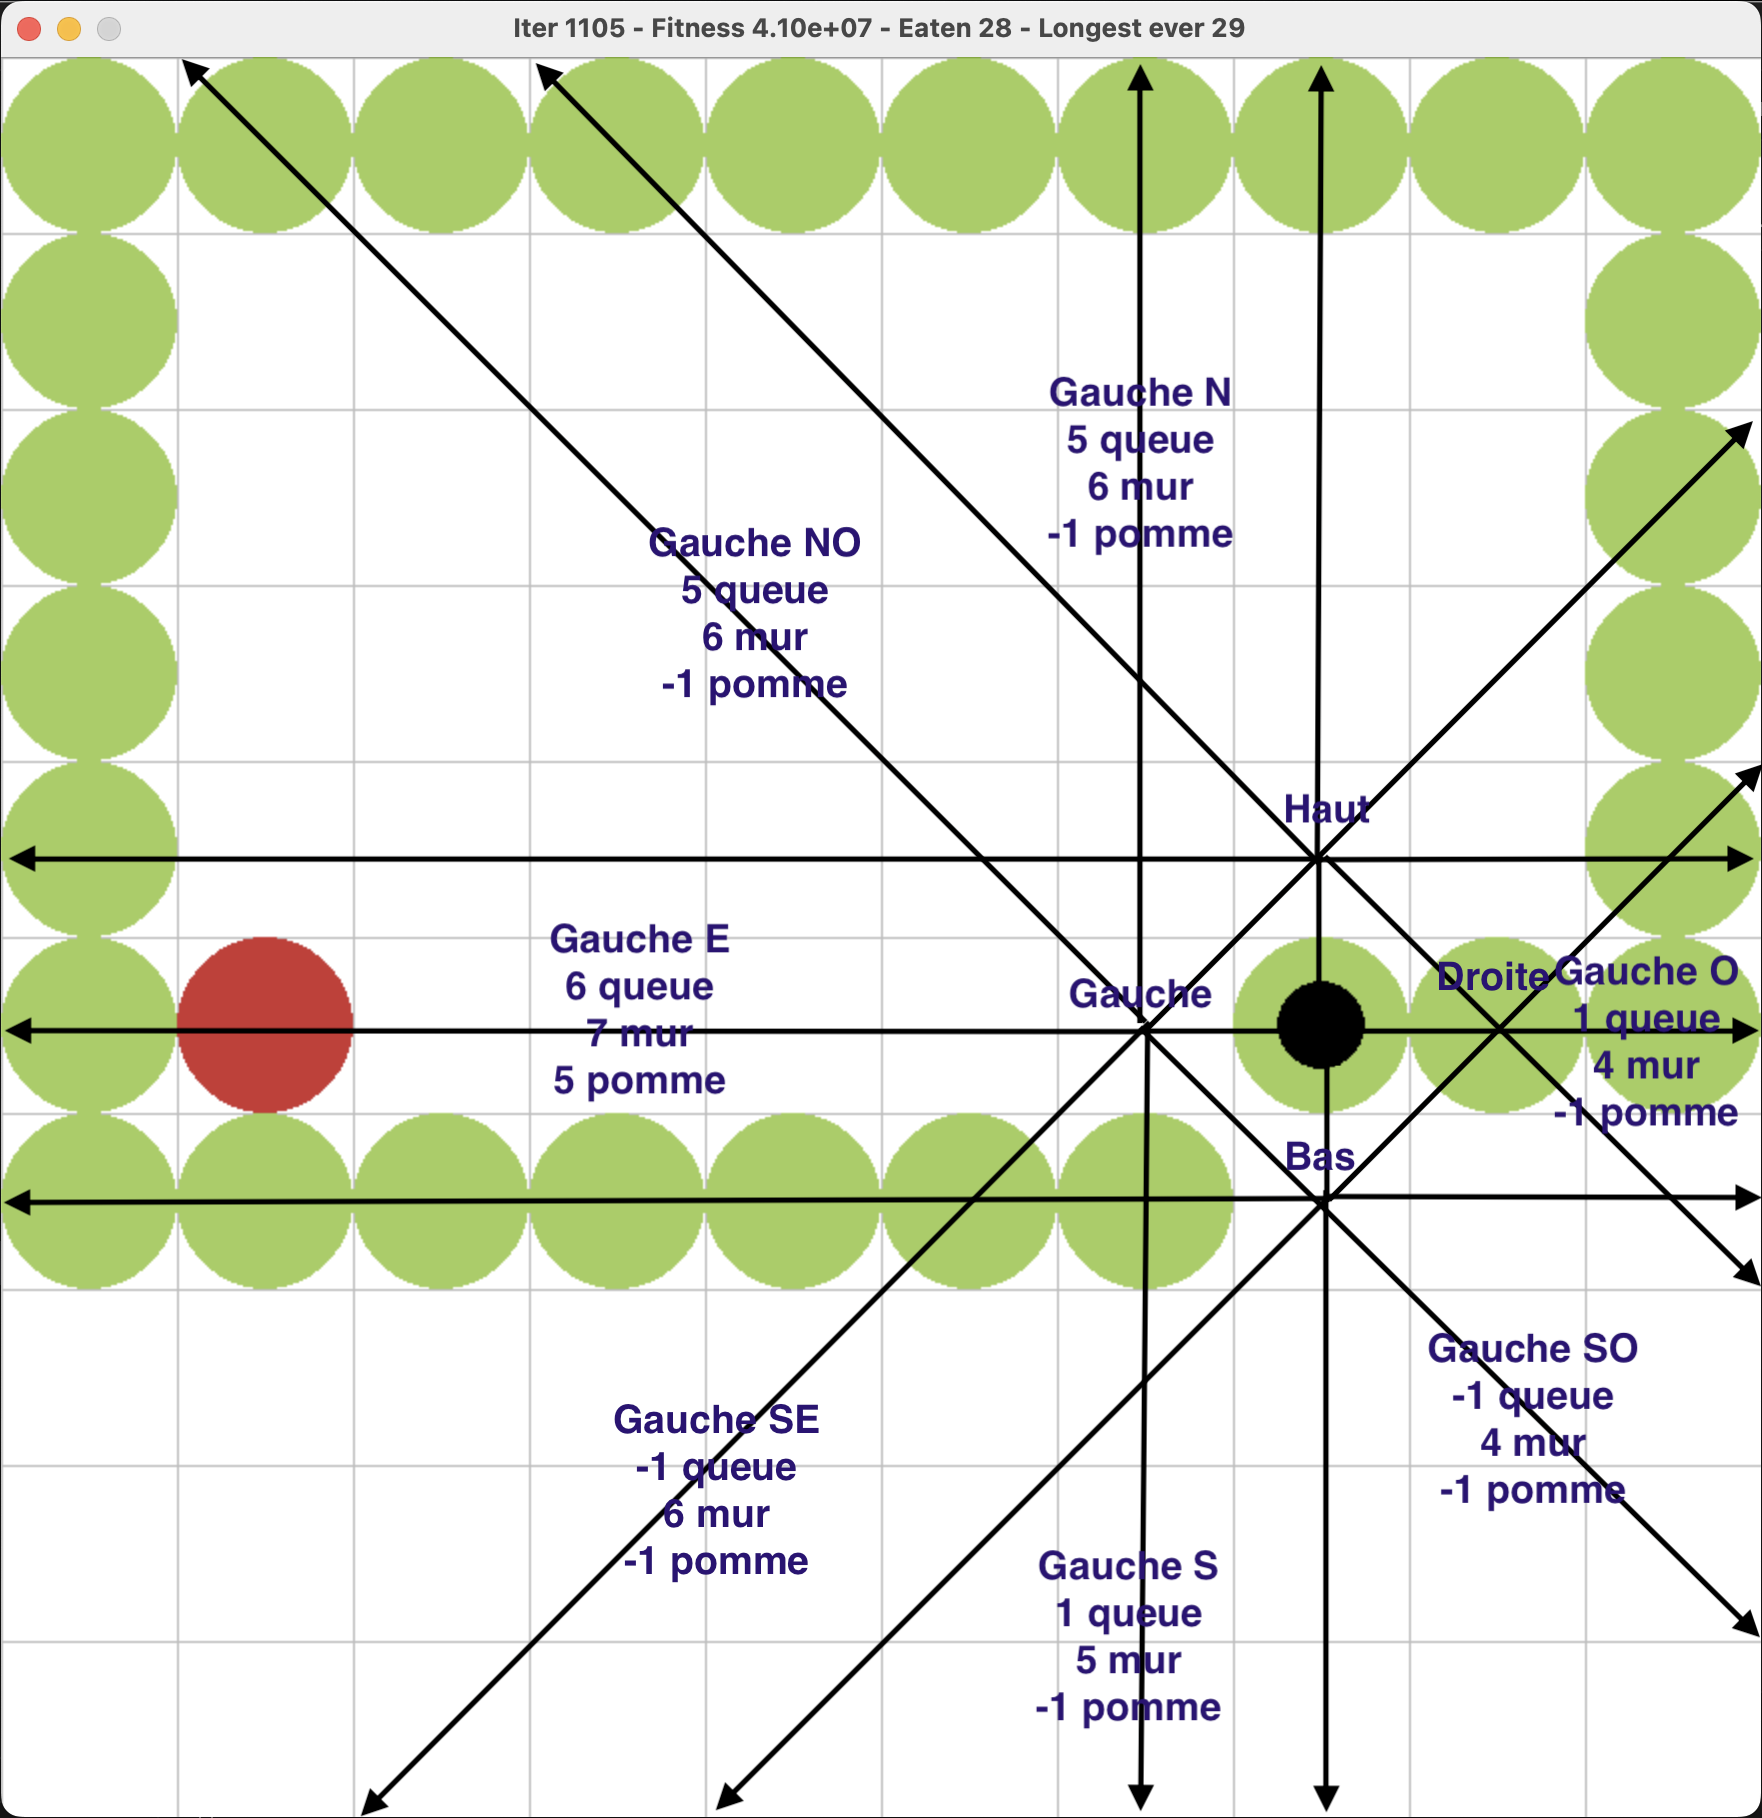
\includegraphics[width=1\textwidth]{snake_vision_illustration2.png}
\vspace{-0.7cm}
\caption*{\tiny Stratégie n\textsuperscript{o} 1}
\end{figure}

\begin{figure}
\vspace{-0.8cm}
%\hspace{-0.6cm}
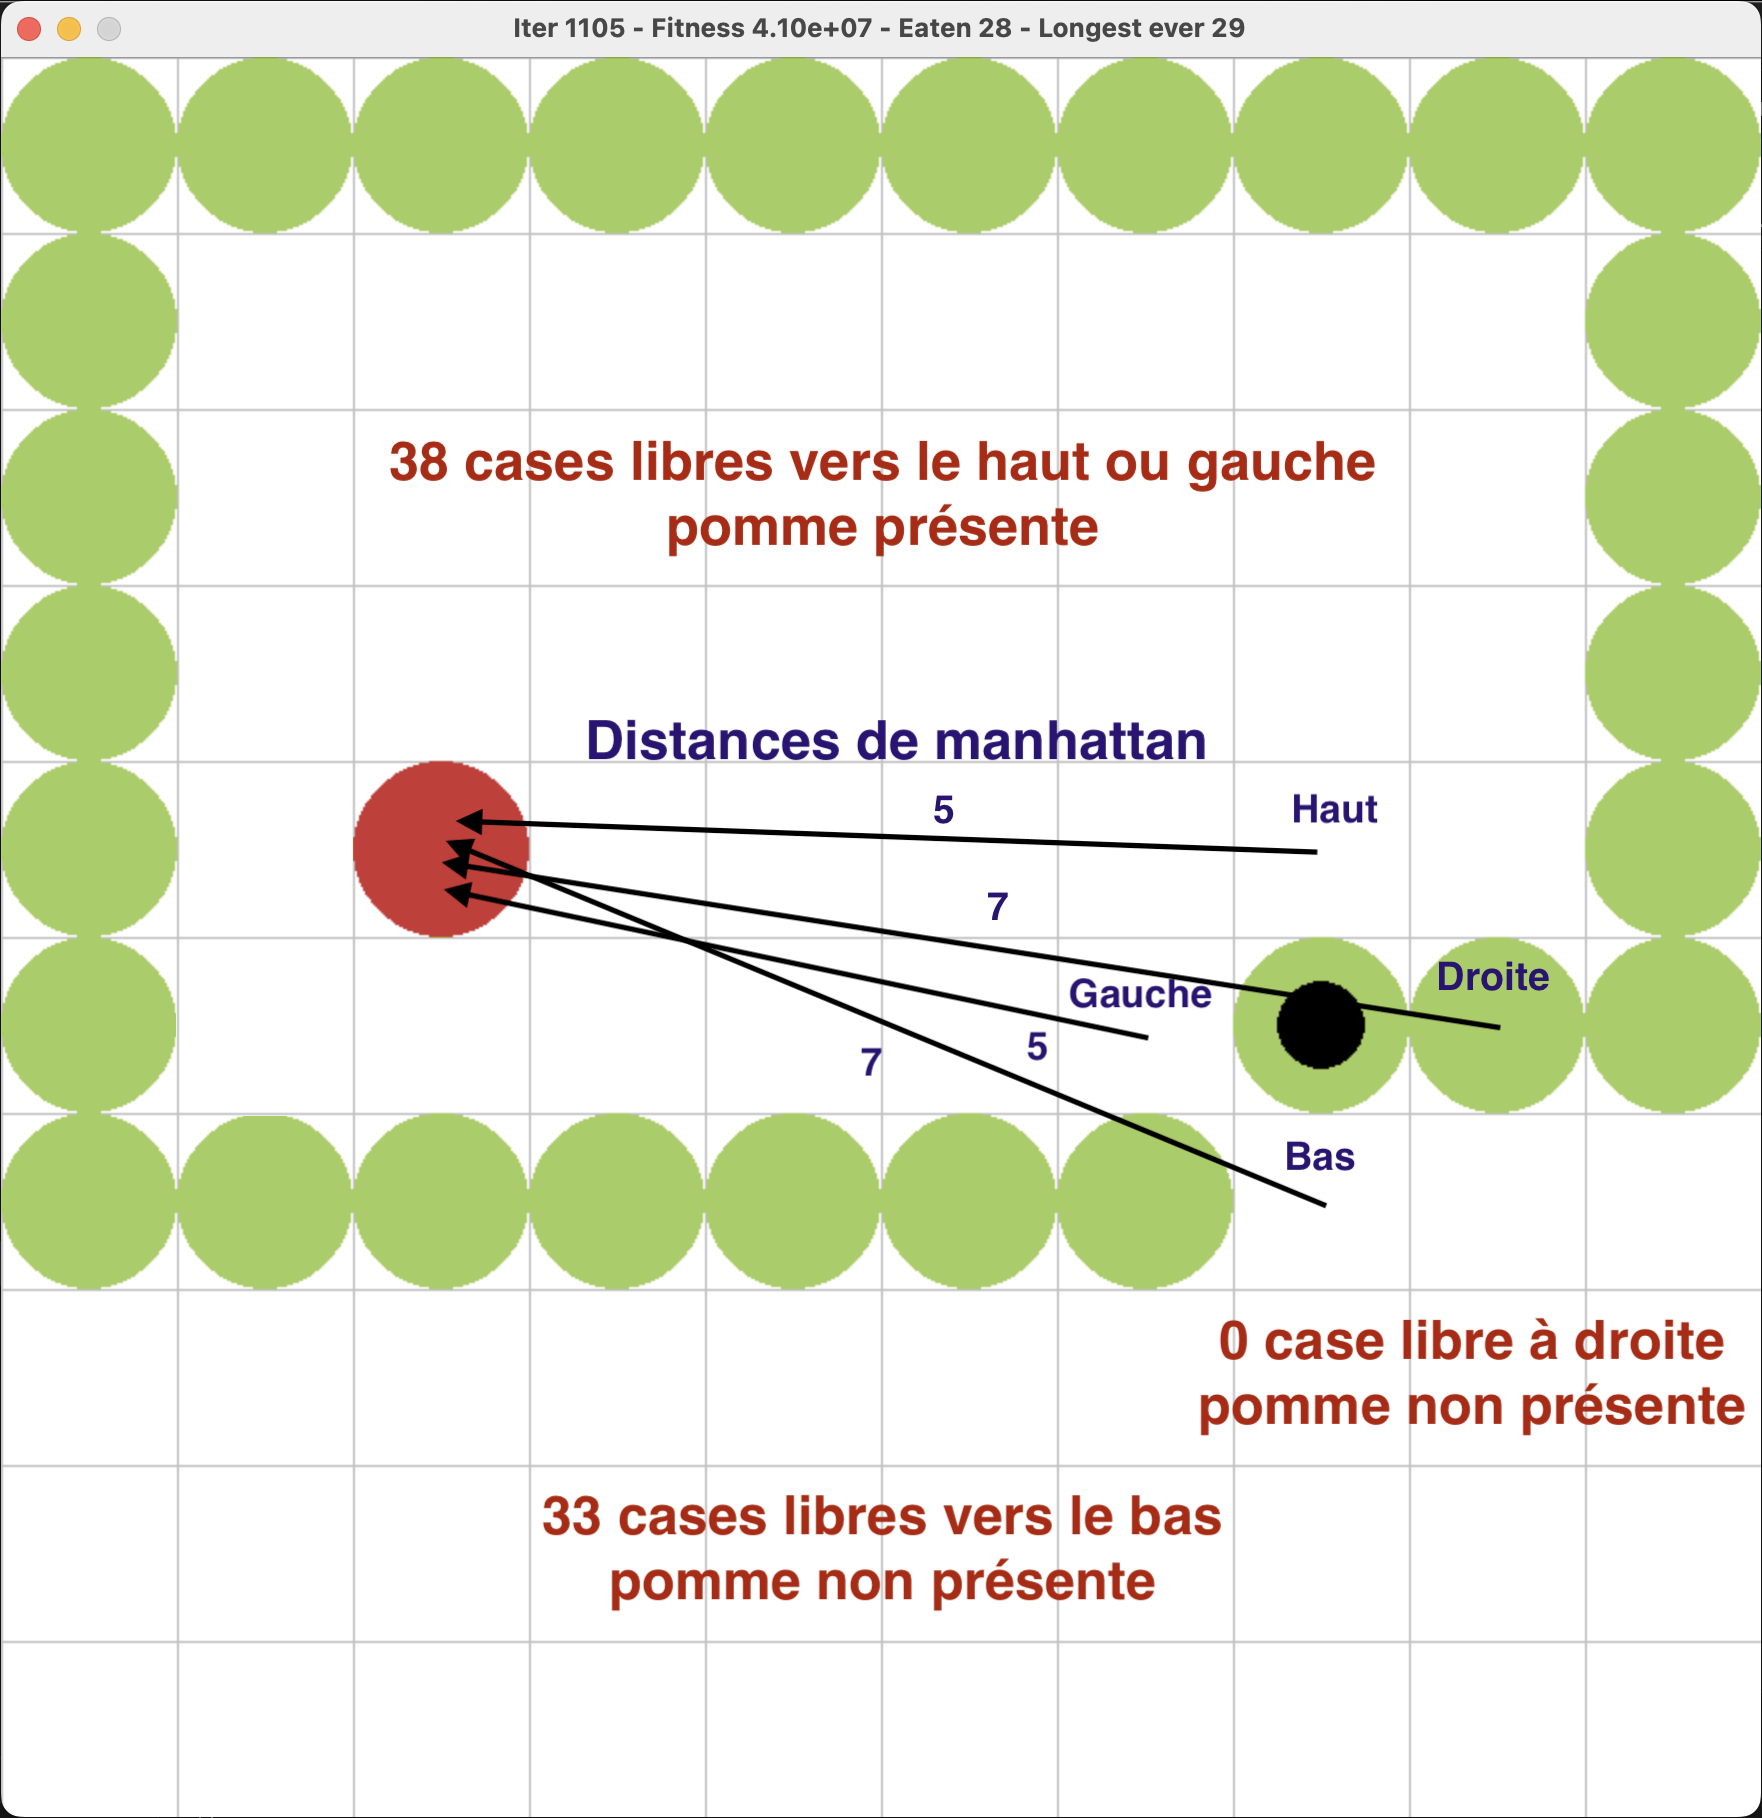
\includegraphics[width=1\textwidth]{snake_vision_illustration.png}
\vspace{-0.7cm}
\caption*{\tiny Stratégie n\textsuperscript{o} 2}
\end{figure}

\end{column}
\end{columns}
\end{frame}

\section{Algorithme génétique}

\subsection{Performance}

\begin{frame}
\frametitle{\'Evaluation de la performance d'un serpent}
\begin{columns}[T]
\begin{column}{0.60\textwidth}
\footnotesize
\textbf{Objectif:} mesurer la performance d'un serpent grâce à une fonction de fitness.

\vspace{0.1cm}
\textbf{Paramètres:} taille du serpent (pommes mangées) et âge (mouvements effectués) à la fin du jeu.

\vspace{0.1cm}
\textbf{Fonctions de fitness évaluées:} maximiser $f_1$ ou $f_2$ favorise la croissance et la longévité des serpents.
\begin{itemize}
  \footnotesize
  \item $f_1(\text{taille}, \text{age})=\text{taille}^3\times \text{age}$
  \item $f_2(\text{taille}, \text{age})=(2\times\text{taille})^2\times \text{age}^{1.5}$
\end{itemize}
\textbf{Astuces:}
\begin{itemize}
  \footnotesize
  \item \textbf{Pour éviter les boucles infinies:} un nombre de points de vie est attribué à chaque serpent, décrémenté à chaque mouvement et réinitialisé à chaque pomme mangée. \'A 0, le serpent meurt et son âge est pénalisé dans le calcul de la fitness.
  \item \textbf{Pour favoriser une croissance rapide:} $f_1$ est utilisée au début du jeu. Ensuite on passe à $f_2$ qui valorise la survie du serpent pour manger plus de pommes.
\end{itemize}

\end{column}

\begin{column}{0.40\textwidth}
\begin{figure}
\centering
\vspace{-0.5cm}
%\hspace{-0.6cm}
\resizebox{\textwidth}{!}{
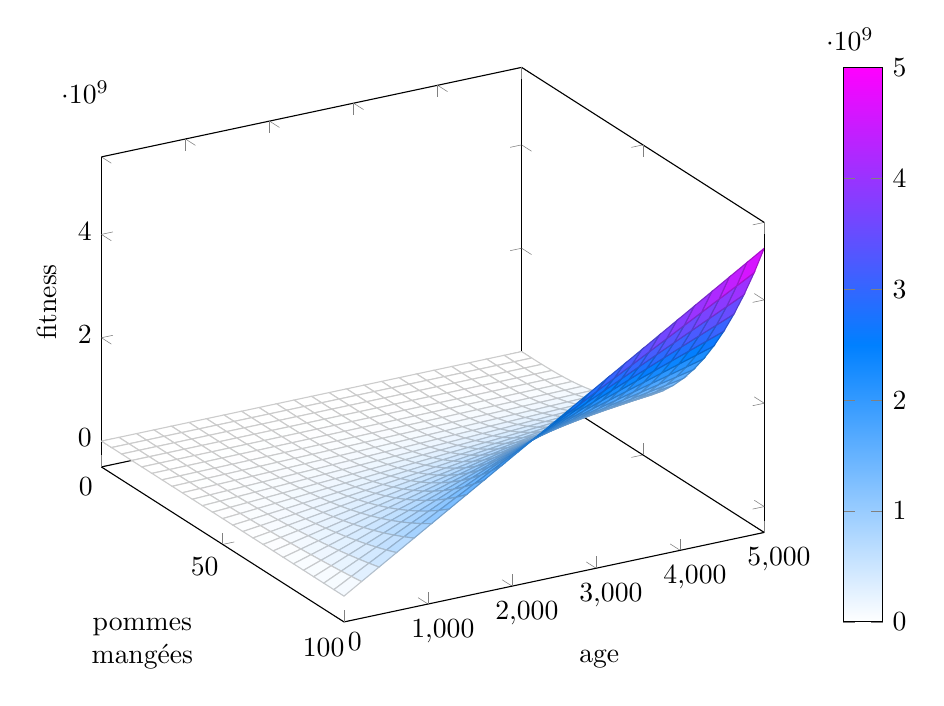
\begin{tikzpicture}
    \begin{axis}[
        width=10cm,
        view={60}{30},
        xlabel={\shortstack{pommes \\ mangées}},
        ylabel={age},
        zlabel={fitness},
        colormap/cool,
        colorbar,
    ]
        \addplot3[
            surf,
            domain=0:100,
            domain y=0:5000,
        ]
        {x^3 * y};
    \end{axis}
\end{tikzpicture}
}
\vspace{-0.4cm}
\caption*{\tiny fitness $f(\text{taille}, \text{age})=\text{taille}^3\times \text{age}$}
\end{figure}

\begin{figure}
\centering
\vspace{-0.5cm}
%\hspace{-0.6cm}
\resizebox{\textwidth}{!}{
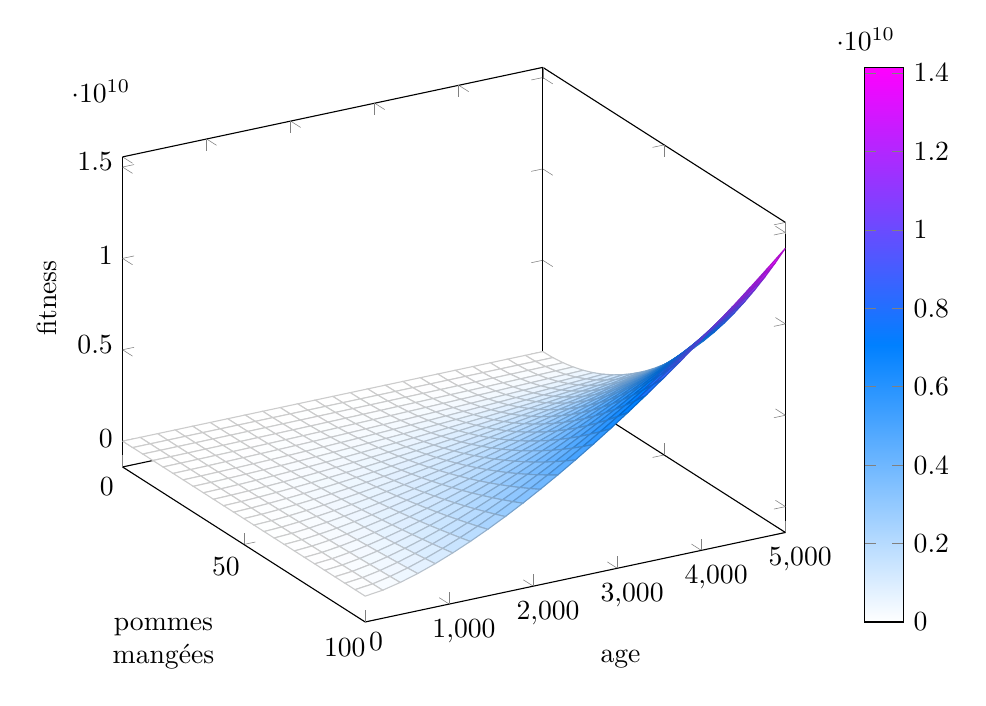
\begin{tikzpicture}
    \begin{axis}[
        width=10cm,
        view={60}{30},
        xlabel={\shortstack{pommes \\ mangées}},
        ylabel={age},
        zlabel={fitness},
        colormap/cool,
        colorbar,
    ]
        \addplot3[
            surf,
            domain=0:100,
            domain y=0:5000,
        ]
        {(x*2)^2 * (y^1.5)};
    \end{axis}
\end{tikzpicture}
}
\vspace{-0.4cm}
\caption*{\tiny fitness $f(\text{taille}, \text{age})=(2\times\text{taille})^2\times \text{age}^{1.5}$}
\end{figure}

\end{column}
\end{columns}
\end{frame}

\subsection{Optimisation}

\begin{frame}
\frametitle{Optimiser les décisions du serpent}
\framesubtitle{Entrainement du réseau de neurones par algorithme génétique}
\begin{columns}[T]
\begin{column}{0.60\textwidth}
\footnotesize

\textbf{Principe:} approche évolutionniste d'une population de réseaux de neurones par algorithme génétique opérant en 3 phases:
\begin{itemize}
  \item \textbf{Sélection:} choix d'une portion individus les plus adaptés pour la reproduction, basé sur leur score de fitness (ici $20\%$).
  \item \textbf{Croisement:} parmis ces serpents sélectionnés, aléatoirement par paires (parents), ils sont recombinés à l'aide d'une technique de croisement en K points (ici K=2) pour recomposer la population totale.
  \item \textbf{Mutation:} ajustement mineur aléatoire dans le chromosome de chaque serpent pour maintenir la diversité.
\end{itemize}

\textbf{Formalisation de la mutation:} $p_m=0.1$ probabilité de mutation, $c_m=0.1$ le coefficient de mutation, $\forall h_i(t)$ à l'itération $t$, on tire $U \sim \mathcal{U}(0, 1)$ et $C \sim \mathcal{U}(-1, 1)$. Si $U<p_m$, $h_i(t+1)=h_i(t)+C\times c_m$ sinon $h_i(t+1)=h_i(t)$.
\end{column}

\begin{column}{0.40\textwidth}

\begin{figure}
\centering
%\vspace{-1cm}
%\hspace{-0.6cm}
\resizebox{\textwidth}{!}{
\tikzset{
  frame/.style={
    rectangle, draw,
    text width=6em, text centered,
    minimum height=4em,drop shadow,fill=lime!40,
    rounded corners,
  },
  line/.style={
    draw, -latex',rounded corners=3mm,
  }
}
\begin{tikzpicture}[font=\small\sffamily\bfseries,very thick,node distance = 4cm]
\node [frame] (pop) {Population};
\node [above=2cm, left of=pop] (init) {Initialisation};
\node [below=2cm, left of=pop] (term) {Fin};
\node [frame, above=2cm, right of=pop] (parents)  {Parents};
\node [frame, below=2cm, right of=pop] (off)  {Enfants};

\path [line] (parents)
 -- node[right,align=left,pos=.5] {Croisement\\[3mm]Mutation}
 (off);
\path [line] (init) |- (pop.170);
\path [line] (pop.190) -| (term);
\path [line] (off) -| node[below,pos=.25, align=center] {Sélection\\ survivants}(pop);
\path [line] (pop) |- node[above,pos=.75, align=center] {Sélection\\ parents}(parents);
\end{tikzpicture}
}
%\vspace{-0.2cm}
\caption*{\tiny Processus itératif}
\end{figure}

\begin{figure}
\centering
%\vspace{-0.7cm}
%\hspace{-0.6cm}
\resizebox{\textwidth}{!}{
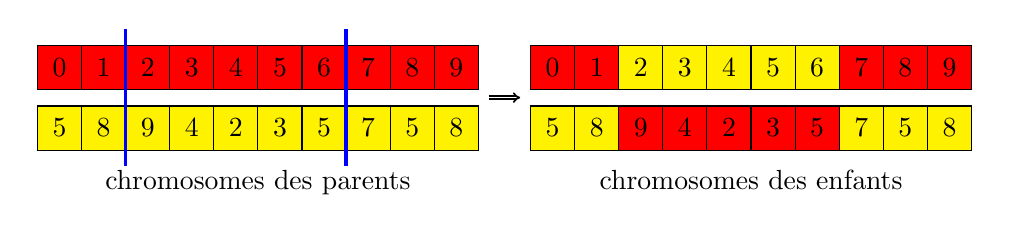
\begin{tikzpicture}[ampersand replacement=\&,  % <-- Add this line for Beamer compatibility
  node distance=4mm,
  MTRX/.style={matrix of nodes,
               nodes={draw, minimum size=5.6mm, anchor=center,
                      inner sep=0pt, outer sep=0pt},
               column sep=-\pgflinewidth,
               row sep=2mm},
  CR/.style={fill=red},
  CY/.style={fill=yellow}
]

% left table
\matrix (m1) [MTRX,
              row 1/.append style={nodes={CR}},
              row 2/.append style={nodes={CY}},
              label=below:chromosomes des parents
             ]
{
0 \& 1 \& 2 \& 3 \& 4 \& 5 \& 6 \& 7 \& 8 \& 9 \\
5 \& 8 \& 9 \& 4 \& 2 \& 3 \& 5 \& 7 \& 5 \& 8 \\
};

% right table
\matrix (m2) [MTRX, right=of m1,
              label=below:chromosomes des enfants
             ]
{
 |[CR]| 0 \& |[CR]| 1 \& |[CY]| 2 \& |[CY]| 3 \& |[CY]| 4 \&
 |[CY]| 5 \& |[CY]| 6 \& |[CR]| 7 \& |[CR]| 8 \& |[CR]| 9 \\
 |[CY]| 5 \& |[CY]| 8 \& |[CR]| 9 \& |[CR]| 4 \& |[CR]| 2 \&
 |[CR]| 3 \& |[CR]| 5 \& |[CY]| 7 \& |[CY]| 5 \& |[CY]| 8 \\
};

\draw[very thick, blue] ([yshift=2mm]m1-1-2.north east) -- ([yshift=-2mm]m1-2-2.south east);
\draw[very thick, blue] ([yshift=2mm]m1-1-7.north east) -- ([yshift=-2mm]m1-2-7.south east);
\draw[double, -{Implies[]}, semithick] (m1.east) -- (m2.west);
\end{tikzpicture}
}
%\vspace{-0.2cm}
\caption*{\tiny Croisement 2 points (2 points crossover)}
\end{figure}
\footnotesize
\textbf{Remarque:} il est garantit que la fitness est améliorée à chaque génération mais pas la convergence vers un optimum global sauf statistiquement.
\end{column}
\end{columns}
\end{frame}

\section{Simulations}

\subsection{Algorithme}

\begin{frame}
  \begin{columns}[T]
  \begin{column}{0.70\textwidth}
  \frametitle{Algorithme d'entrainement résultant}
  \framesubtitle{Entrainement par algorithme générique\\ d'un réseau de neurones pour jouer à Snake}
  \begin{algorithmic}
    \tiny
      \State Population $\mathcal{P}$ $\gets 484=22^2$ serpents
      \ForAll{serpent $s \in \mathcal{P}$}
          \State cerveau $c$ de $s$ $\gets$ réseau neurones $\left[13, 12, 12, 4\right]$, poids \& biais aléatoires
      \EndFor
      \State génération $g \gets 0$
      \While{$g < 2000$}
          \For{serpent $s \in \mathcal{P}$}
              \State age $a_s \gets 0$ de $s$, longeur $l_s \gets 3$, point de vie $v_s \gets 50$
              \State vivant $\gets$ true, $\text{mortVieillesse}_s \gets$ false
              \While{vivant}
                  \State $\text{position}_s \gets$ avance direction $=c\left[\text{vision}_s\left(\text{position}_s\right)\right]$
                  \If{$\text{position}_s \in \left\{\text{mur}, \text{queue}\right\} \text{or } v_s<0$}
                      \State $\text{vivant}_s =$ false
                  \Else
                      \State $a_s \gets a_s + 1$
                  \EndIf
                  \If{$\text{position}_s \in \left\{\text{pomme}\right\}}$
                      \State $l_s \gets l_s + 1$, $v_s \gets 50$
                      \State regénère pomme emplacement aléatoire accessible
                  \Else
                      \State $v_s \gets v_s - 1$
                  \EndIf
                  \If{$v_s<0$}
                      \State $\text{mortVieillesse}_s \gets$ true
                  \EndIf
              \EndWhile
              \State $\text{fitness}_s \gets f_s(l_s, a_s, \text{mortVieillesse}_s)$
          \EndFor
          \State $S \gets 20\%$ des meilleurs serpents au sens de $\text{fitness}_s$
          \State Reconstitue $\mathcal{P} \gets S \bigcup \text{mutations}\left[\text{croisements}(S)\right]$
          \State $g \gets g + 1$
      \EndWhile
  \end{algorithmic}

  \end{column}
  \begin{column}{0.26\textwidth}
  \begin{figure}
  \centering
  \vspace{-2.0cm}
  %\hspace{-0.6cm}
  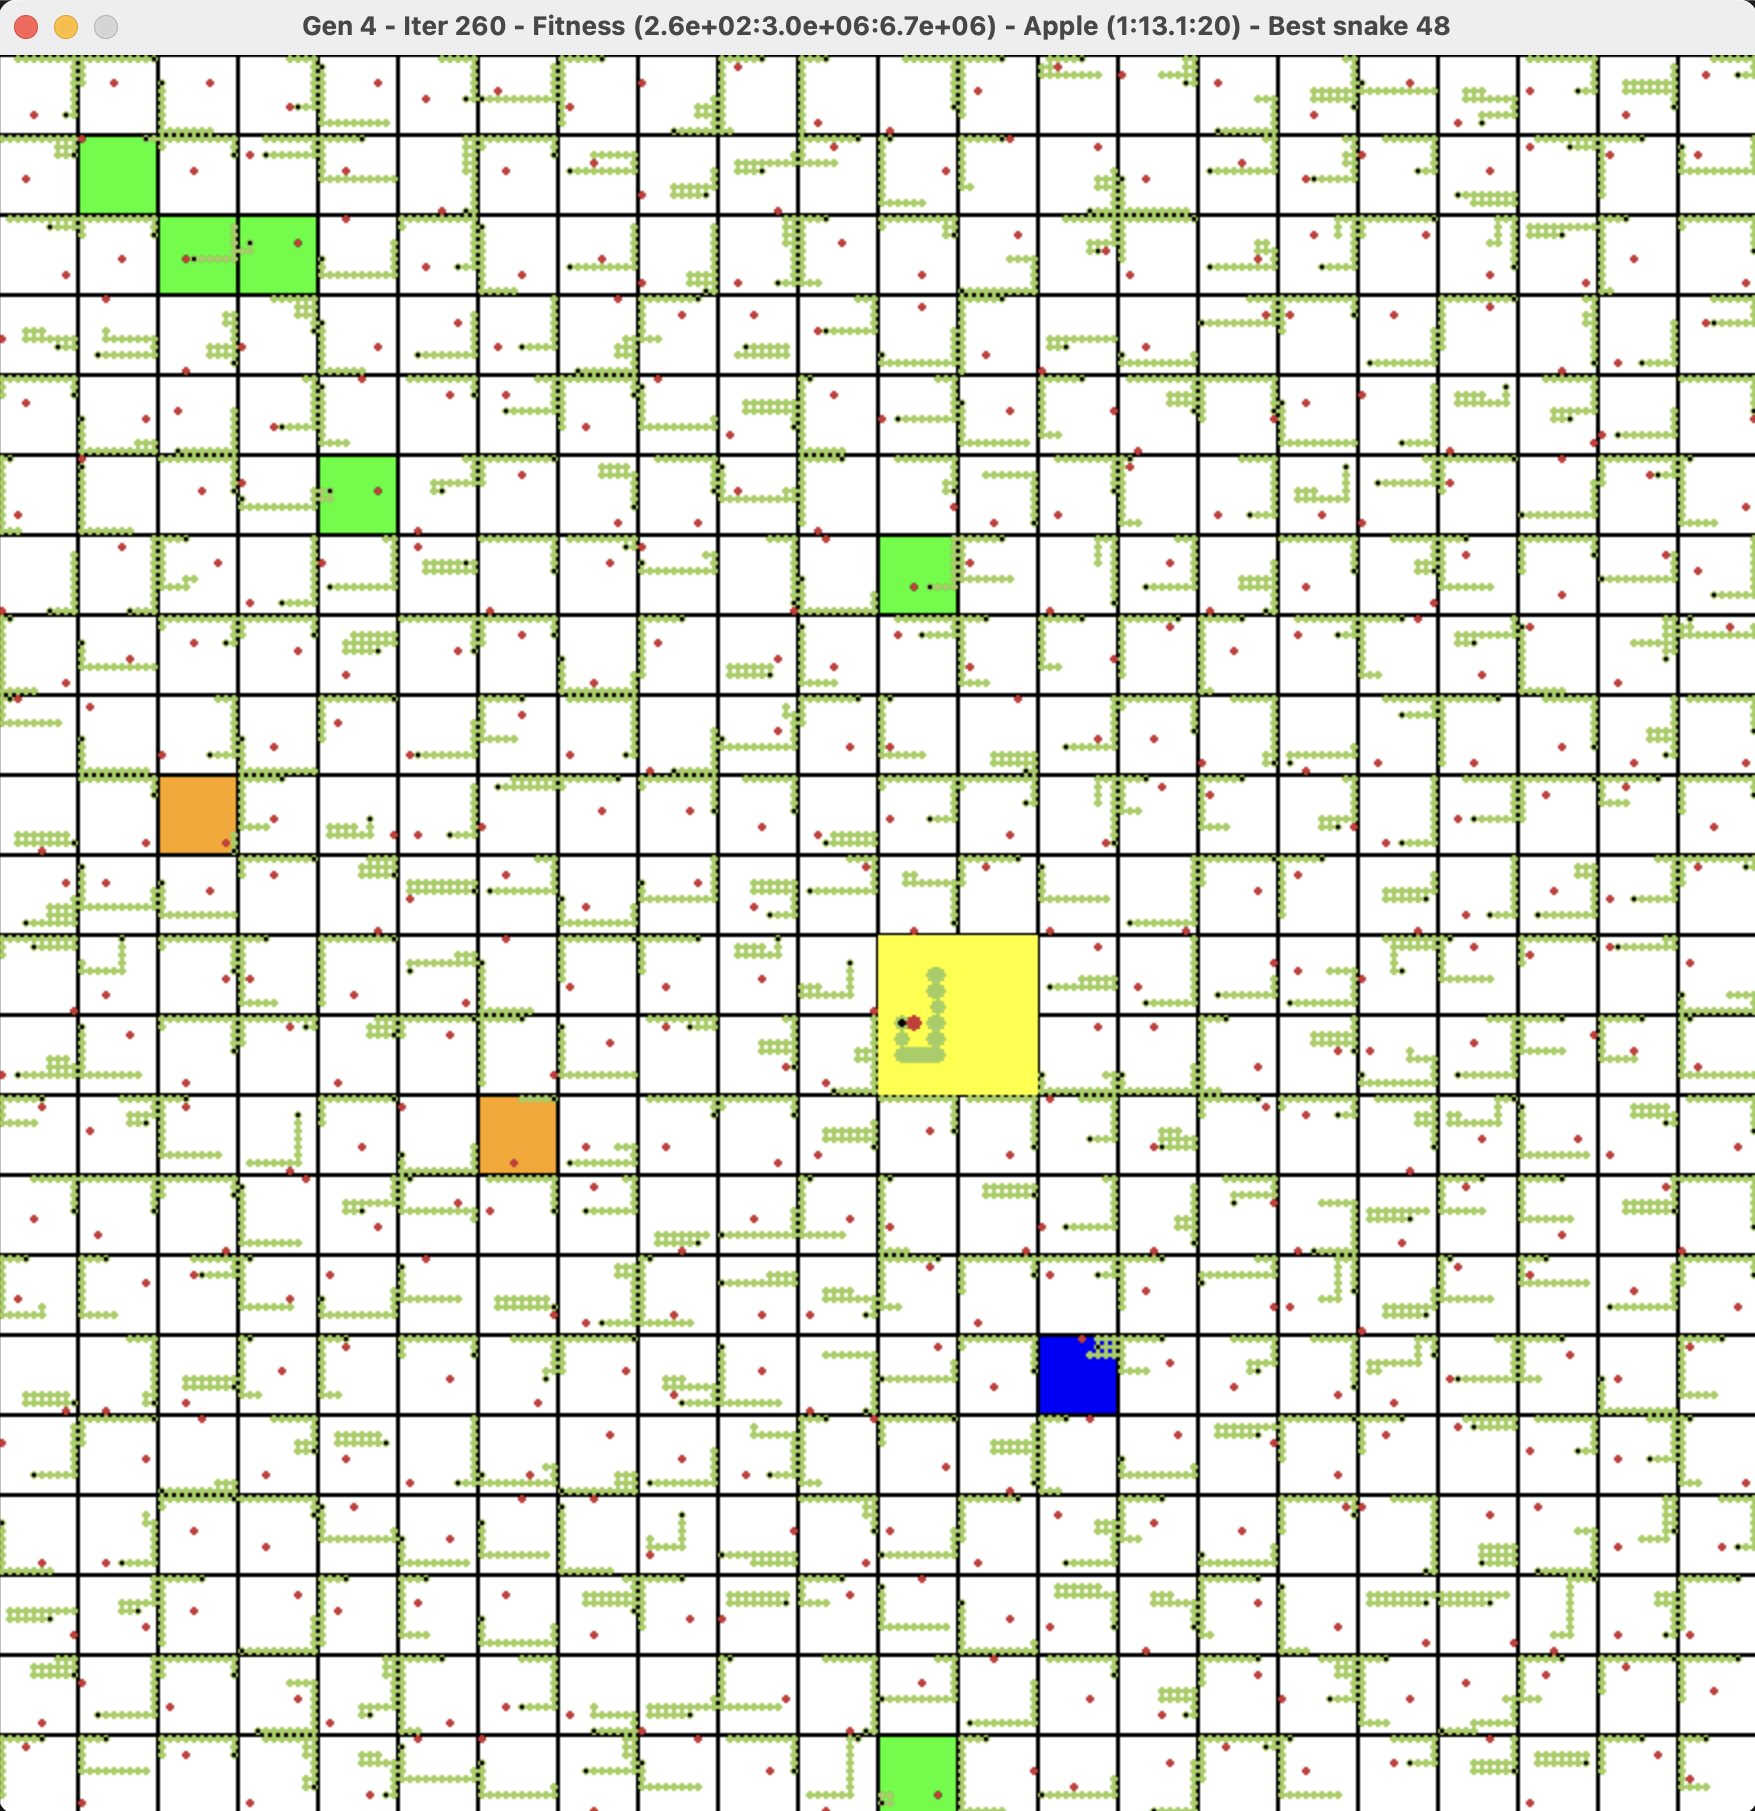
\includegraphics[width=1\textwidth]{snake_population.png}
  \vspace{-0.7cm}
  \caption*{\tiny Population de serpents}
  \end{figure}

  \begin{figure}
  \centering
  \vspace{-0.6cm}
  %\hspace{-0.6cm}
  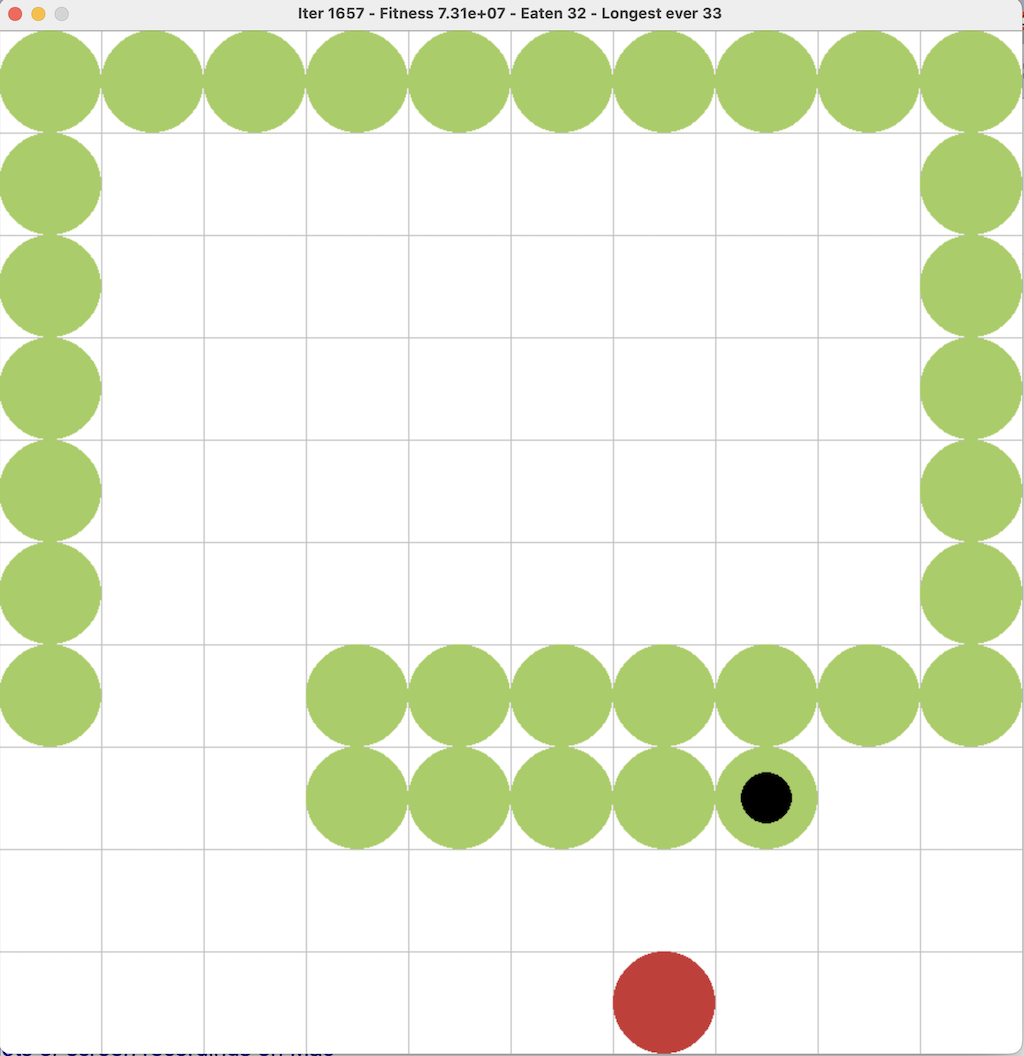
\includegraphics[width=1\textwidth]{snake_game.png}
  \vspace{-0.7cm}
  \caption*{\tiny Le jeu pour un serpent}
  \end{figure}

  \begin{figure}
  \centering
  \vspace{-0.6cm}
  %\hspace{-0.6cm}
  % NEURAL NETWORK
  \resizebox{\textwidth}{!}{
  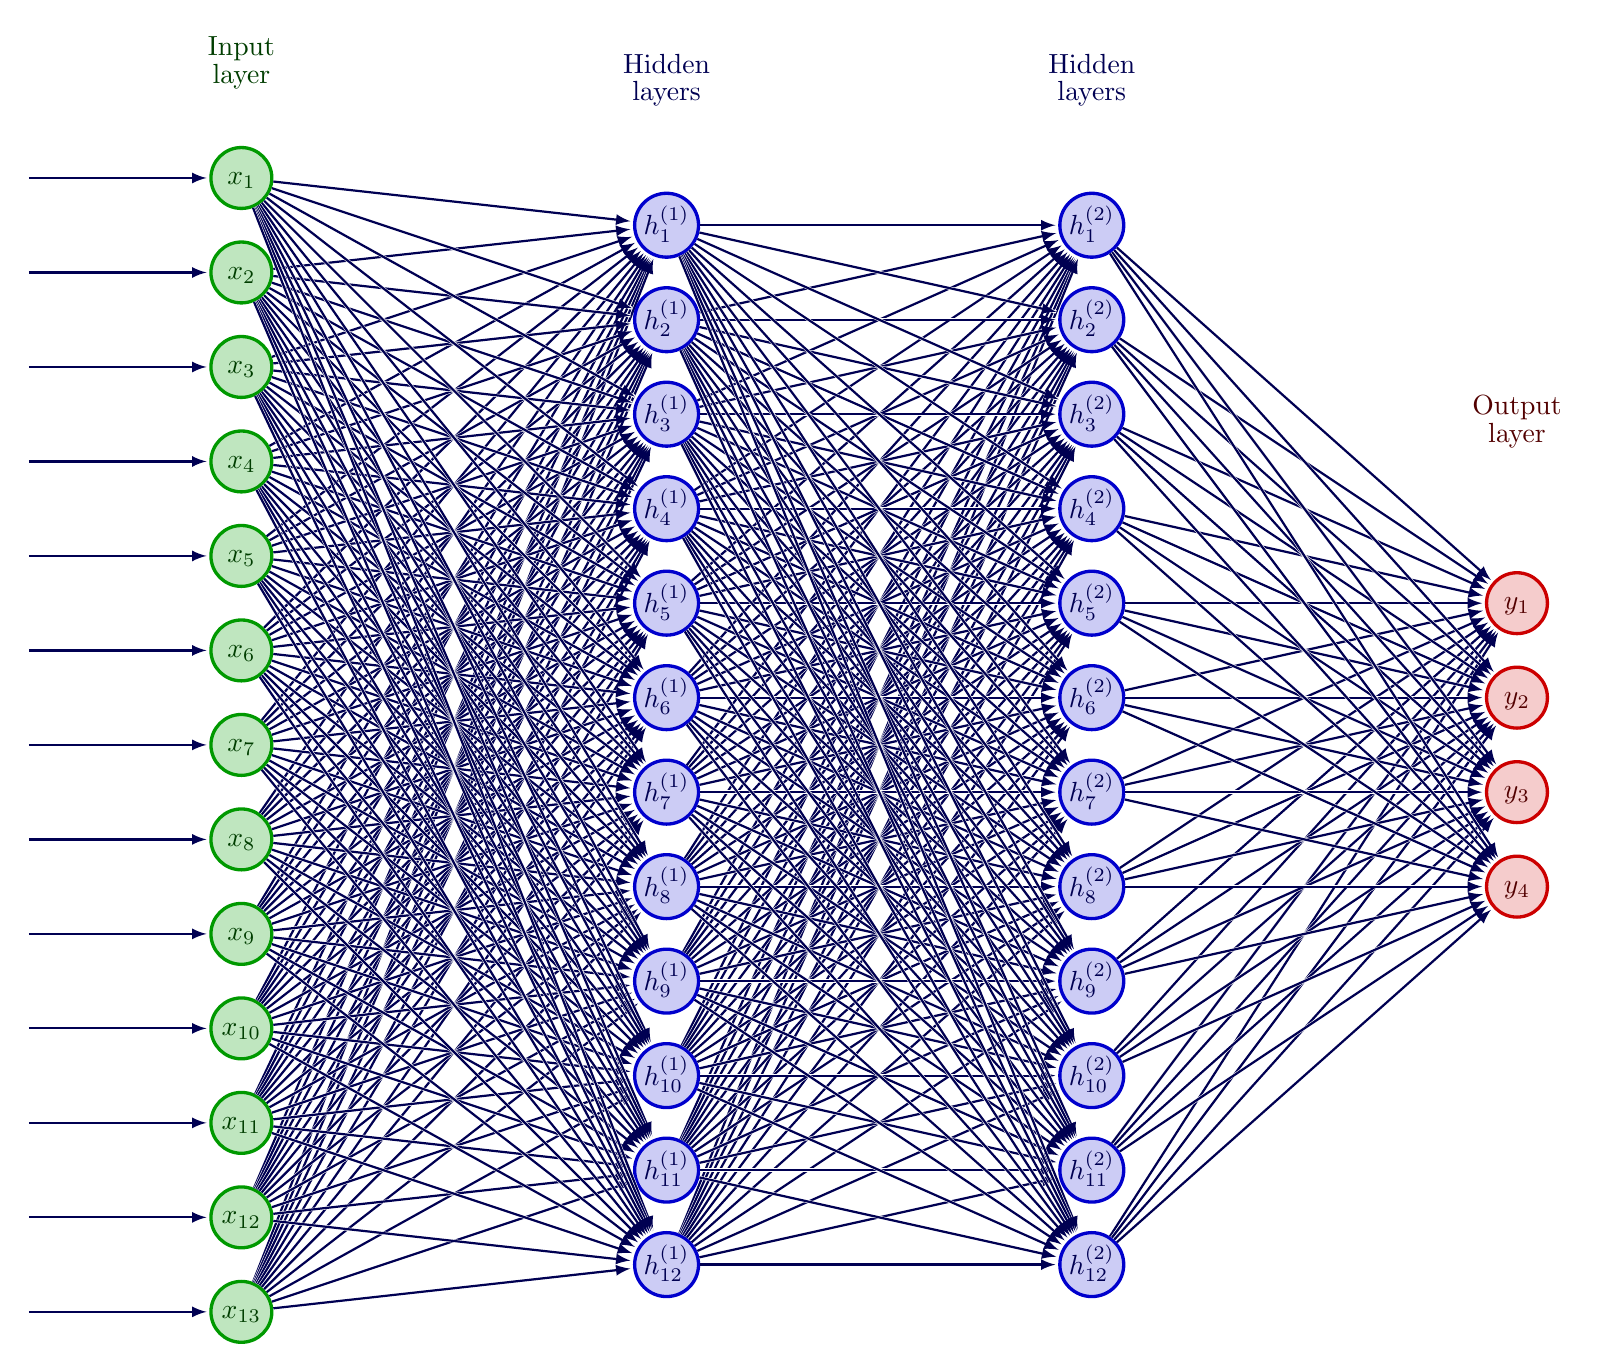
\begin{tikzpicture}[x=5.4cm,y=1.2cm]
    \readlist\Nnod{13,12,12,4}
    \readlist\Nstr{13,12,4} % array of string number of nodes per layer
    \readlist\Cstr{x,h^{(\prev)},y} % array of coefficient symbol per layer
    \def\yshift{0.55} % shift last node for dots
    % Calculate the maximum number of nodes in any layer
    \def\maxN{0}
    \foreachitem \X \in \Nnod{
      \ifnum\X>\maxN
        \xdef\maxN{\X}
      \fi
    }
    % LOOP over LAYERS
    \foreachitem \N \in \Nnod{
      \def\lay{\Ncnt} % alias of index of current layer
      \pgfmathsetmacro\prev{int(\Ncnt-1)} % number of previous layer
      \pgfmathsetmacro\midY{(\N-1)/2} % midpoint of the current layer
      \foreach \i [evaluate={\c=int(\i==\N); \y=\midY-\i; % Adjusted \y calculation
                   \x=\lay; \n=\nstyle;
                   \index=(\i<\N?int(\i):"\Nstr[\n]");}] in {1,...,\N}{ % loop over nodes
        % NODES
        \node[node \n] (N\lay-\i) at (\x,\y) {$\strut\Cstr[\n]_{\index}$};

        % CONNECTIONS
        \ifnumcomp{\lay}{>}{1}{ % connect to previous layer
          \foreach \j in {1,...,\Nnod[\prev]}{ % loop over nodes in previous layer
            \draw[white,line width=1.2,shorten >=1] (N\prev-\j) -- (N\lay-\i);
            \draw[connect] (N\prev-\j) -- (N\lay-\i);
          }
        }{
          \draw[connect] (0.5,\y) -- (N\lay-\i); % arrows in
        }
      }
    }
    % LABELS
    \node[above=0.5,align=center,mydarkgreen] at (N1-1.north) {Input\\[-0.2em]layer};
    \node[above=0.8,align=center,mydarkblue] at (N2-1.north) {Hidden\\[-0.2em]layers};
    \node[above=0.8,align=center,mydarkblue] at (N3-1.north) {Hidden\\[-0.2em]layers};
    \node[above=1.2,align=center,mydarkred] at (N4-1.north) {Output\\[-0.2em]layer};
  \end{tikzpicture}
  } % End of \resizebox
  \vspace{-0.7cm}
  \caption*{\tiny Cerveau du serpent stratégie n$\textsuperscript{o}$5}
  \end{figure}

  \end{column}
  \end{columns}
\end{frame}

\subsection{Convergence}

\begin{frame}
\frametitle{Résultats de convergence}
\begin{figure}
\vspace{-0.3cm}
%\hspace{-0.6cm}
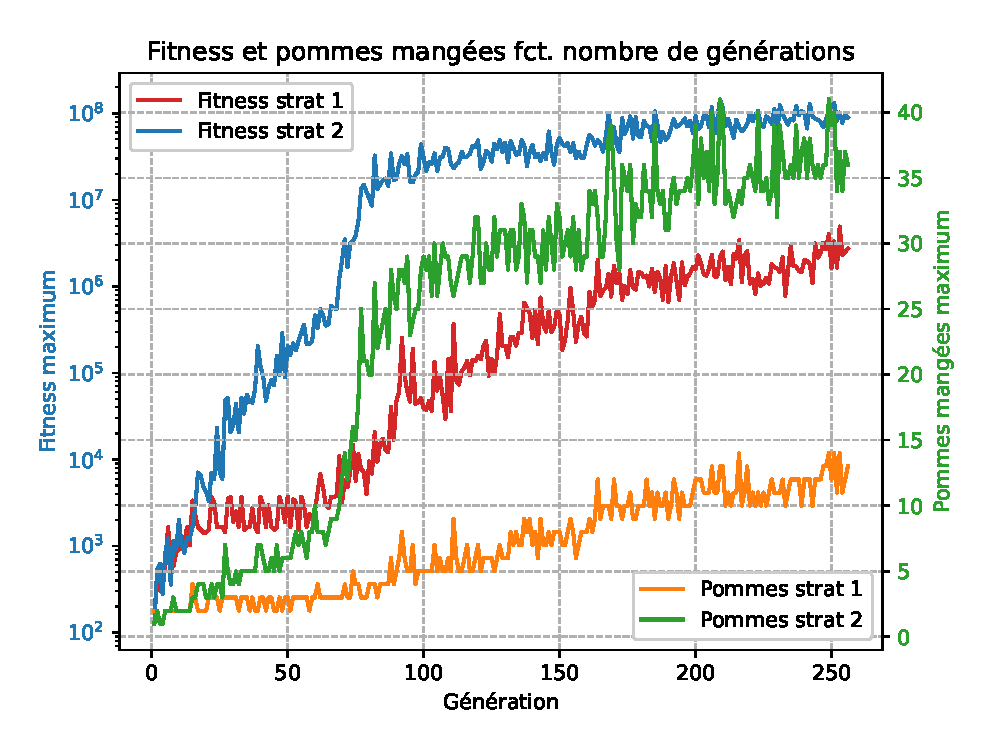
\includegraphics[width=0.8\textwidth]{curve_compare_cv.eps}
\vspace{-0.4cm}
\caption*{\tiny Convergence des stratégies de vision n$\textsuperscript{o}$1 et n$\textsuperscript{o}$5}
\end{figure}
\vspace{-0.4cm}
\begin{itemize}
\footnotesize
\item \textbf{Observations:} la stratégie de vision n$\textsuperscript{o}$5 converge plus rapidement que la stratégie n$\textsuperscript{o}$1, et atteint un score de fitness plus élevé.
\item \textbf{Interprétation:} la stratégie de vision n$\textsuperscript{o}$5 fournit au serpent des informations plus pertinentes pour localiser la pomme et anticiper ses mouvements sans s'en retrouver prisonnier.
\end{itemize}

\end{frame}

\section{Conclusion}

\begin{frame}
\frametitle{Conclusion}
\footnotesize
\begin{itemize}
\item Deux outils mathématiques de modélisation et d'optimisation mis en \oe{}uvre pour résoudre le problème de jeu de Snake:
  \begin{itemize}
  \item des réseaux de neurones afin de prendre des décisions de mouvements dont les entrées sont des informations visuelles du serpent sur le jeu.
  \item des algorithmes génétiques pour optimiser les poids et biais des réseaux de neurones.
  \end{itemize}
\item Différentes stratégies de vision et de fitness ont été proposées et discutées en terme de pertinence et performance.
\item Des pistes d'améliorations restent à explorer:
  \begin{itemize}
  \item Optimisation de la conception du réseau de neurones.
  \item Utiliser une fonction de fitness dynamique pour mieux prendre en compte les contraintes de la taille du serpent.
  \end{itemize}
\item Tous les programmes ont été implémentés en python avec une interface graphique pygame permettant une visualisation en temps réel de l'optimisation de la population de serpents.
% code from scratch
\item La totalité du projet est disponible en annexes et sur github: \url{https://github.com/marilabs/tipe-2024}
\end{itemize}
\end{frame}

\end{document}

\section{Annexe I: \textbf{Snake game: code en python}}

\begin{frame}[t,allowframebreaks]{Configuration}{config.py}
\scriptsize
\inputminted[mathescape]{python}{../../snake-the-game/config.py}
\end{frame}

\begin{frame}[t,allowframebreaks]{Un jeu}{game.py}
\scriptsize
\inputminted[mathescape]{python}{../../snake-the-game/game.py}
\end{frame}

\begin{frame}[t,allowframebreaks]{La population: collection de jeux}{game\_collection.py}
\scriptsize
\inputminted[mathescape]{python}{../../snake-the-game/game_collection.py}
\end{frame}

\begin{frame}[t,allowframebreaks]{Algorithme génétique}{genetic\_algorithm.py}
\scriptsize
\inputminted[mathescape]{python}{../../snake-the-game/genetic_algorithm.py}
\end{frame}

\begin{frame}[t,allowframebreaks]{Réseau de neurones}{neural\_network.py}
\scriptsize
\inputminted[mathescape]{python}{../../snake-the-game/neural_network.py}
\end{frame}

\begin{frame}[t,allowframebreaks]{Programme principal}{main.py}
\scriptsize
\inputminted[mathescape]{python}{../../snake-the-game/main.py}
\end{frame}

\begin{frame}[t,allowframebreaks]{Rejouer le meilleur serpent sauvé}{play\_snake.py}
\scriptsize
\inputminted[mathescape]{python}{../../snake-the-game/play_snake.py}
\end{frame}

\begin{frame}[t,allowframebreaks]{Courbes de convergence}{plot\_compare\_convergences.py}
\scriptsize
\inputminted[mathescape]{python}{../../snake-the-game/plot_compare_convergences.py}
\end{frame}

\section{Annexe II: \textbf{Snake game: jeu jouable par l'utilisateur}}

\begin{frame}[t,allowframebreaks]{Jeu intéractif}{playable\_game.py}
\scriptsize
\inputminted[mathescape]{python}{../../snake-the-game/playable-snake/playable_game.py}
\end{frame}

\begin{frame}[t,allowframebreaks]{Programme principal du jeu intéractif}{playable\_main.py}
\scriptsize
\inputminted[mathescape]{python}{../../snake-the-game/playable-snake/playable_main.py}
\end{frame}

\end{document}

\begin{frame}
\frametitle{Améliorations et astuces}
\end{frame}

\begin{frame}
\frametitle{Titre}
\framesubtitle{Sous-titre}
\begin{columns}[T]
\begin{column}{0.70\textwidth}
\footnotesize
\textbf{Point:} blah
\vspace{0.5cm}
\textbf{Point:}
\begin{itemize}
\footnotesize
\item toto
\item tutu
\end{itemize}
\end{column}
\begin{column}{0.24\textwidth}
\begin{figure}
\centering
\vspace{-1cm}\hspace{-0.6cm}
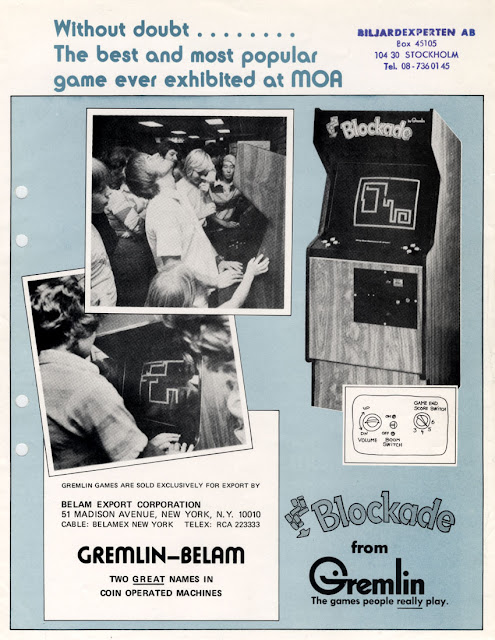
\includegraphics[width=1\textwidth]{blockade.jpg}
\caption*{\tiny toto}
\end{figure}
\end{column}
\end{columns}
\end{frame}

\begin{frame}
  TODO

  Breadth-First Search (BFS) algorithm to count free spaces in each direction
  Optimisation pour recalculer récursivement à chaque itération

  Mutation is necessary to prevent the population from being stuck at a local maximum.

  chrommosome enfant

  TODO: choix en design du réseau de neurones

  ICI: max des sorties donne la direction

  vocabulaire: génération (itération)

  pousser la simulation à 2000 itérations

  Normalement Minimiser erreur quadratique moyenne, mais sorties non déterministes et séquence.
  Descente de gradient.
  Trop de possibilités.
  Là pas possible.
  Reenforcement learning.
  Choix Algo génétique.

  Se déplacer grace à un réseau de neurones.
  Déplacements régis par un réseau de neurones
  Optimiser le déplacement grace à un algorithme génétique.

  Serpent point de vie, age et taille

  Eviter les boucle infinie: décrémenter les points de vies, restaurer les points de vie dès qu'on mange une pomme, appliquer une pénalité au score en décrémentant age par 50 si mort de vieillesse

  * The number of hidden neurons should be between the size of the input layer and the size of the output layer.
  * The number of hidden neurons should be 2/3 the size of the input layer, plus the size of the output layer.
  * The number of hidden neurons should be less than twice the size of the input layer.
  * The number of hidden neurons should be between the size of the input layer and the output layer.
  * The most appropriate number of hidden neurons is sqrt(input layer nodes * output layer nodes)
  \end{frame}


\subsection{L'algorithme génétique}
\begin{frame}
\frametitle{Le principe de l'algorithme génétique}
\framesubtitle{Histoire, fonctionnement et applications de l'algorithme}
\begin{itemize}
\item \textbf{Origines:} développé par John Holland dans les années 1970
\item \textbf{Principe:} s'inspirer de l'évolution naturelle pour
    résoudre des problèmes d'optimisation
\item \textbf{Fonctionnement:} on part d'une population aléatoire, on les fait évoluer en appliquant des opérateurs
    génétiques (sélection, crossover, mutation)
\item \textbf{Applications:} problème du voyageur de commerce, problèmes de décision (optimisation dans les banques), NASA et Sony pour des déplacements de robots, automatisation des tests d'application par Motorola

\item \textbf{Ici:} application ludique, on applique cet algorithme à un réseau neuronal pour qu'il joue à Snake
\end{itemize}
\end{frame}

\subsection{Les réseaux neuronaux}

\begin{frame}

  \frametitle{Le principe des réseaux neuronnaux}
  \framesubtitle{Histoire et principe}

  \begin{itemize}

    \item \textbf{Origines:} Warren S. McCulloch et Walter Pitts, \textit{A logical calculus of the ideas immanent in nervous activity}, 1943, compare les neurones à seuil binaire à la logique booléenne puis Frank Rosenblatt, \textit{The perceptron: a probabilistic model for information storage and organization in the brain}, 1958, introduit la notion de poids

    \item \textbf{Principe:} 3 couches de n\oe uds qui transmettent des informations à la couche suivante suivant s'ils sont activés et leurs poids, s'appuient sur l'entraînement pour être plus précis

    \item \textbf{Fonctionnement:} on code des "yeux" au serpent, ie. on prend en compte ce qu'il voit devant lui, et le réseau neuronal va analyser ces données pour que le serpent tourne ou pas.

    \item \textbf{Lien avec l'algorithme génétique:} les différents poids associés aux neurones vont être transmis ou non aux enfants

  \end{itemize}

  \end{frame}

  \section{La théorie}


  \subsection{L'algorithme génétique}

  \begin{frame}
    \frametitle{Le fonctionnement de l'algorithme génétique}
  \end{frame}

  \begin{frame}
    \frametitle{Le Théorème de Holland}
  \end{frame}

  \subsection{Les réseaux neuronaux}


\section{L'algorithme appliqué au jeu de Snake}

\subsection{Relation algorithme génétique et réseaux de neurones}

\begin{frame}
  \frametitle{Comment algorithme génétique et réseaux de neurones sont reliés}

\end{frame}

\subsection{L'importance d'une fonction de fitness: trouver la bonne stratégie}

\begin{frame}
  \frametitle{Trouver la stratégie gagnante avec la fonction fitness}
\end{frame}

\subsection{Les résultats}

\begin{frame}
  \frametitle{Les résultats}
\end{frame}

\end{document}

\begin{frame}
  \frametitle{Algorithme d'entrainement résultant}
  \framesubtitle{Entrainement par algorithme générique d'un réseau de neurones pour jouer à Snake}
  \footnotesize
  \textbf{Principe:}
  \begin{itemize}
  \footnotesize
  \item On part d'une large population composée de $484=22^2$ serpents.
  \item Chaque serpent évolue sur son propre plateau de jeu.
  \item Le cerveau de chaque serpent est un réseau de neurones dont les entrées sont des paramètres de visions et dont les sorties fournissent les 4 décisions de directions \keystroke{$\leftarrow$}\keystroke{$\uparrow$}\keystroke{$\downarrow$}\keystroke{$\rightarrow$}.
  \end{itemize}
  \textbf{\'Etapes de l'algorithme:}
  \begin{itemize}
  \footnotesize
  \item Initialisation: tous les réseaux de neurones sont initialisés avec des poids aléatoires.
  \item Itération: Tous les serpents de la population évoluent dans le jeu jusqu'à ce qu'ils meurent en heurtant un mur, mangeant leur queue ou s'il n'ont pas manger de pomme pendant un nombre donné d'itérations (pour éviter les boucles infinies).
  \item Mesure: \`A tout jeu on associe un "score" ou fonction de fitness dépendant de sa taille et du nombre de mouvements total effectués sans mourir
  \item Sélection: seul un pourcentage des meilleurs serpents sont retenus (ici $10\%$) au sens du score de fitness.
  \item \'Evolution: ces meilleurs serpents sont utilisés pour reconstituer la population totale par croisement et mutation entre deux des meilleurs serpents tirés au hasard.
  \end{itemize}}
\end{frame}
